% =====================================================================================
%  Cristal sónico de LEGO — relatório LFE (Módulo I)
%  Compilar: pdflatex relatorio.tex (2×). Figuras 2–3 e tabela do apêndice: python fazer_figuras.py
%  Texto a vermelho (\confirmar{...}) = dados que não estão nos ficheiros: confirmar e depois
%  trocar a definição de \confirmar para \newcommand{\confirmar}[1]{#1}.
% =====================================================================================
\documentclass[10pt,twocolumn,a4paper]{article}
\usepackage[utf8]{inputenc}
\usepackage[T1]{fontenc}
\usepackage{lmodern}
\usepackage[portuguese]{babel}
\usepackage[a4paper,top=1.45cm,bottom=1.6cm,left=1.45cm,right=1.45cm,columnsep=0.55cm]{geometry}
\usepackage{amsmath,amssymb}
\usepackage{graphicx}
\usepackage{booktabs}
\usepackage{xcolor}
\usepackage{tikz}
\usetikzlibrary{decorations.pathreplacing}
\usepackage[font=footnotesize,labelfont=bf,labelsep=period,skip=3pt]{caption}
\usepackage{titlesec}
\usepackage{enumitem}
\usepackage{microtype}
\usepackage{longtable}
\usepackage[hidelinks]{hyperref}

\newcommand{\confirmar}[1]{\textcolor{red}{#1}}   % depois de confirmar: {#1}
\newcommand{\GX}{\Gamma X}
\newcommand{\GM}{\Gamma M}
\newcommand{\finf}{f_\text{inf}}
\newcommand{\fsup}{f_\text{sup}}
\newcommand{\fc}{f_\text{c}}

\titleformat{\section}{\normalsize\bfseries}{\thesection}{0.5em}{}
\titlespacing*{\section}{0pt}{5pt plus 2pt}{2pt}
\titleformat{\subsection}{\small\bfseries}{\thesubsection}{0.5em}{}
\titlespacing*{\subsection}{0pt}{4pt}{1pt}
\setlength{\parskip}{0pt}
\setlength{\textfloatsep}{6pt plus 2pt}
\setlength{\floatsep}{5pt plus 2pt}
\setlength{\abovedisplayskip}{3pt}\setlength{\belowdisplayskip}{3pt}
\setlength{\abovedisplayshortskip}{2pt}\setlength{\belowdisplayshortskip}{2pt}
\renewcommand{\refname}{Referências}
\pagestyle{plain}

\begin{document}
\twocolumn[{%
\begin{center}
  {\Large\bfseries Hiatos de Bragg num cristal sónico de LEGO nas direções $\GX$ e $\GM$}\\[4pt]
  {\small Filipe Marcelino (ist1117896) e \confirmar{[nome da colega] (ist1xxxxxx)}
   \;·\; LFE, Módulo I \;·\; \confirmar{Grupo X} \;·\; Instituto Superior Técnico, outubro de 2026}
\end{center}
\vspace{-2pt}
\noindent\colorbox{black!6}{\parbox{\dimexpr\textwidth-2\fboxsep}{\small
\textbf{Resumo.}
Medimos a transmissão de ruído branco através de uma rede quadrada de colunas LEGO $2{\times}2$
(lado $s=15{,}8$\,mm, passo $a=32$--$56$\,mm, $N=1$--$11$ filas), ao longo de $\GX$ e de $\GM$, e
comparámos o hiato com uma expansão em ondas planas (PWE) de um cristal 2D de hastes rígidas.
Em $\GX$, o bordo de baixo concorda com a PWE para $a\le48$\,mm:
$\finf=3806\pm84$, $3586\pm151$ e $2969\pm102$\,Hz contra $3892$, $3387$ e $2988$\,Hz ($z\le1{,}3$);
para $a=56$\,mm os dois bordos ficam ${\approx}10\,\%$ acima ($z\approx4$).
O hiato não escala como $1/a$: o centro passa de $(0{,}904\pm0{,}018)\,f_B$ a $(1{,}094\pm0{,}022)\,f_B$ e a reta
$\fc\propto1/(2a)$ dá $\chi^2/\nu=15$.
A profundidade cresce linearmente com $N$, com ordenada na origem compatível com zero, a
$\alpha=1{,}45\pm0{,}29$ a $1{,}98\pm0{,}41$\,dB/fila ($a=40$--$56$\,mm), 50--80\,\% da PWE, e satura em
${\approx}13$--$15$\,dB por som que contorna o cristal.
Em $\GM$, $\finf$ fica 8--11\,\% abaixo da PWE ($z=2{,}5$--$3{,}6$) e o hiato não fecha por cima,
porque a difração lateral começa em $f_B$; $\finf(\GM)/\finf(\GX)=1{,}36\pm0{,}06$ ($a=48$\,mm), entre
$\sqrt2$ e a PWE ($1{,}47$). Não há evidência de hiato completo, como a PWE prevê.}}
\vspace{8pt}
}]

% =====================================================================================
\section{Introdução}
Um cristal sónico é uma rede periódica de obstáculos rígidos no ar. As reflexões em planos
de obstáculos sucessivos, separados por $d$, somam-se em fase quando $\lambda=2d$, e à volta de
\begin{equation}
  f_B=\frac{c}{2d},\qquad d=a\ (\GX),\qquad d=a/\sqrt2\ (\GM)
\end{equation}
abre-se um hiato de banda~\cite{martinez1995,kushwaha1993}: no bordo da zona de Brillouin,
$k=\pi/d$, as ondas estacionárias com a pressão máxima nos planos de tijolos e no ar entre eles
deixam de ter a mesma frequência, e entre as duas, $\finf<f_B<\fsup$, nenhuma onda se propaga.
Dentro do hiato $k=\pi/d+i\kappa$ e a pressão decai como $e^{-\kappa x}$; ao fim de $N$ filas a
atenuação em decibéis é
\begin{equation}
  D(N)=\alpha N,\qquad \alpha=20\log_{10}(e)\,\kappa d .
  \label{eq:DN}
\end{equation}
A posição e a largura do hiato dependem da fração de enchimento $f\!f=s^2/a^2$ ($0{,}24$ a $0{,}08$
aqui): os tijolos tornam o som mais lento, $c_\text{ef}\simeq c/\sqrt{1+f\!f}$~\cite{krokhin2003}, e o
hiato desce abaixo de $f_B$, tanto mais quanto menor for $a$. As bandas calculam-se resolvendo
$\nabla\!\cdot(\rho^{-1}\nabla p)+\omega^2p/(\rho c^2)=0$ com $p$ escrito como onda de Bloch (PWE,
225 ondas planas, Apêndice~B).
Testámos, em $\GX$ e $\GM$, os bordos do hiato, a sua dependência em $a$ e a atenuação linear em $N$,
e se os hiatos das duas direções se sobrepõem (hiato completo).

% =====================================================================================
\section{Método}
\begin{figure}[t]
  \centering
  % Fig. 1 — montagem e esquema de medição (vista de cima, fora de escala)
\resizebox{\columnwidth}{!}{%
\begin{tikzpicture}[x=1cm,y=1cm,
    tij/.style={fill=black!75,draw=none},
    lbl/.style={font=\scriptsize},
    cota/.style={<->,>=stealth,thin}]
  \def\a{0.34}
  \pgfmathsetmacro{\d}{\a/sqrt(2)}
  \pgfmathsetmacro{\L}{\a*sqrt(2)}
  % coluna de som + frentes de onda (comum aos dois painéis)
  \newcommand{\fonte}{%
    \draw[fill=black!15] (0,-0.35) rectangle (0.3,0.35);
    \foreach \r in {0.5,0.65,0.8}
      \draw[black!45,thin] (\r,-0.42) arc[start angle=-35,end angle=35,radius=0.73];
    \draw[->,>=stealth,thick,black!60] (0.62,0.62) -- (1.02,0.62) node[right=-2pt,lbl] {$\mathbf k$};
    \node[lbl] at (0.6,-0.68) {$\approx$70\,cm};
    \node[lbl] at (0.15,0.5) {coluna};
    \fill (3.7,0) circle (0.065);
    \node[lbl] at (3.7,0.27) {mic.};}
  % ---------------------------------------------------------------- (a) ΓX
  \begin{scope}
    \node[lbl,anchor=west] at (-0.05,1.2) {(a) $\Gamma X$:\; $d=L=a$};
    \fonte
    \foreach \i in {0,...,4}
      \foreach \j in {-1.5,-0.5,0.5,1.5}
        \fill[tij] ({1.3+\i*\a-0.075},{\j*\a-0.075}) rectangle ++(0.15,0.15);
    \draw[cota] (1.3,0.78) -- (1.3+\a,0.78) node[midway,above=-2pt,lbl] {$a$};
    \draw[decorate,decoration={brace,amplitude=3pt,mirror}] (1.22,-0.68) -- ({1.3+4*\a+0.08},-0.68)
      node[midway,below=1pt,lbl] {$N$ filas};
    \draw[cota] ({1.3+4*\a+0.08},-0.32) -- (3.7,-0.32) node[midway,below=-1pt,lbl] {5--10\,cm};
  \end{scope}
  % ---------------------------------------------------------------- (b) ΓM
  \begin{scope}[xshift=4.45cm]
    \node[lbl,anchor=west] at (-0.05,1.2) {(b) $\Gamma M$:\; $d=a/\sqrt2$,\; $L=\sqrt2\,a$};
    \fonte
    \foreach \i in {0,...,5} {
      \pgfmathtruncatemacro{\paridade}{mod(\i,2)}
      \ifnum\paridade=0
        \foreach \j in {-1,0,1}
          \fill[tij,rotate around={45:({1.3+\i*\d},{\j*\L})}] ({1.3+\i*\d-0.075},{\j*\L-0.075}) rectangle ++(0.15,0.15);
      \else
        \foreach \j in {-1.5,-0.5,0.5,1.5}
          \fill[tij,rotate around={45:({1.3+\i*\d},{\j*\L})}] ({1.3+\i*\d-0.075},{\j*\L-0.075}) rectangle ++(0.15,0.15);
      \fi
    }
    \draw[cota] (1.3,-0.95) -- ({1.3+\d},-0.95) node[midway,below=-2pt,lbl] {$d$};
    \draw[cota] ({1.3+5*\d+0.2},{0.5*\L}) -- ({1.3+5*\d+0.2},{1.5*\L}) node[midway,right=-2pt,lbl] {$L$};
  \end{scope}
\end{tikzpicture}}

  \caption{Montagem vista de cima (fora de escala). Cada coluna são 4 tijolos $2{\times}2$
  empilhados (3,8\,cm de altura) numa placa LEGO; $a$ é múltiplo de 8\,mm (passo dos pinos).
  (a) $\GX$: 4 colunas de largura. (b) $\GM$: rede rodada $45^\circ$, filas alternadas de 4 e 3
  tijolos. $d$: distância entre planos; $L$: período dentro de um plano. A coluna emite ruído
  branco; a referência é a mesma geometria sem tijolos.}
  \label{fig:montagem}
\end{figure}
O cristal (Fig.~\ref{fig:montagem}) foi montado com $a=32$, 40, 48 e 56\,mm em $\GX$
($N=10\to1$) e $a=32$, 40 e 48\,mm em $\GM$ ($N=11\to1$). Uma coluna Bluetooth, a
\confirmar{${\approx}70$\,cm} da face do cristal (critério de onda plana, Apêndice~B), emite ruído branco
durante 10\,s; um microfone USB \confirmar{5--10\,cm} atrás do cristal grava a 48\,kHz, 5 vezes por
configuração. Cada bloco (um $a$) começa por uma \emph{referência} sem tijolos, segue-se o cristal
com o máximo de filas, e retira-se uma fila de cada vez do lado do microfone, com a coluna e o
microfone presos com fita. Em $\GM$ o bloco acaba com uma segunda referência. Ao todo: 72
configurações, 360 gravações, em 4 sessões (1 e 6/out em $\GX$, 12 e 13/out em $\GM$), a
$T=20{,}5$ e $20{,}0\pm1\,^\circ$C, ou seja $c=343{,}5\pm0{,}6$ e $343{,}2\pm0{,}6$\,m/s.

Dividir pela referência cancela a resposta da coluna, do microfone e da sala:
\begin{equation}
  T(f)=10\log_{10}\frac{\bar P_\text{cristal}(f)}{\bar P_\text{ref}(f)}\ \text{(dB)},
\end{equation}
com $P$ o espectro de Welch~\cite{welch1967} (Hann, 4096 pontos, $\Delta f=11{,}7$\,Hz, troço 0,8--10,3\,s por causa
do atraso do Bluetooth) suavizado em potência em $1/6$ de oitava antes de dividir. Repetições com
saturação ou cortes do Bluetooth são postas de parte.

% =====================================================================================
\section{Análise}
De cada $T(f)$ tira-se: o nível base $T_0$ (mediana na banda de controlo $0{,}35$--$0{,}70\,c/(2a)$,
transparente nas duas direções) e a \emph{ondulação} (desvio robusto de $T$ nessa banda, onde $T$
devia ser plano); o hiato, zona contínua com $T<T_0-6$\,dB que toca em $0{,}75$--$1{,}25\,f_B$, cujos
cruzamentos do limiar são $\finf$ e $\fsup$ (o hiato ``fecha'' se $\fsup<1{,}5\,f_B$); e a profundidade
$D=T_0-\langle T\rangle_{f_B\pm10\%}$. As janelas estão em unidades de $f_B$, por isso as contas são
iguais nas duas direções.

\emph{Incertezas.} Para cada número, $\sigma^2=\sigma_\text{est}^2+\sigma_\text{ond}^2+\sigma_\text{ref}^2
(+\sigma_\text{res}^2)$: dispersão das 5 repetições ($/\sqrt5$, quase sempre desprezável), ondulação
propagada ($0{,}92\times$ondulação em $D$; ondulação$/|dT/df|$ nos bordos), dispersão entre as
referências do mesmo dia, e $\Delta f/\sqrt{12}=3{,}4$\,Hz. Por bloco, as frequências são a média
ponderada dos $N\ge4$, com $\sigma^2=\sigma_\text{disp}^2+\sigma_\text{sis}^2$: a parte sistemática
(ondulação e referência, comuns a todo o bloco) não diminui com a média.
Os ajustes são mínimos quadrados ponderados ($\sigma_a=0{,}1$\,mm por variância efetiva); se
$\chi^2/\nu>1$ as incertezas são multiplicadas por $\sqrt{\chi^2/\nu}$. A teoria tem incerteza do lado
do tijolo ($\pm0{,}1$\,mm) e da truncatura da PWE (0,5\,\%). Comparações por
$z=|x-x_0|/\sqrt{\sigma_x^2+\sigma_0^2}$.

% =====================================================================================
\section{Resultados}
\begin{figure}[t]
  \centering
  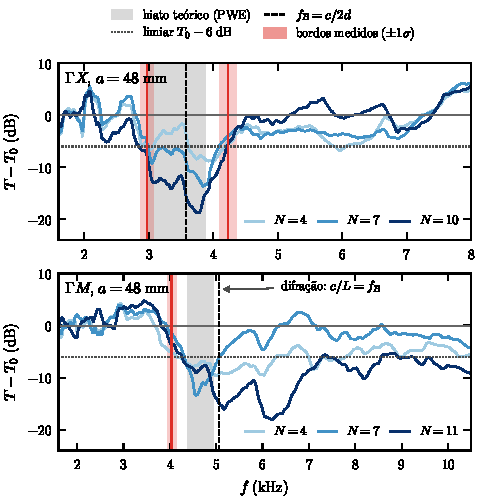
\includegraphics[width=\columnwidth]{figuras/fig2_transmissao.pdf}
  \caption{Transmissão relativa para $a=48$\,mm. Cinzento: hiato da PWE; vermelho: bordos medidos
  (média dos $N\ge4$). Em $\GX$ o hiato fecha; em $\GM$ a difração lateral começa em $f_B$ e $T$
  não volta a 0. Todos os $a$ no Apêndice~A.}
  \label{fig:T}
\end{figure}
\begin{figure}[t]
  \centering
  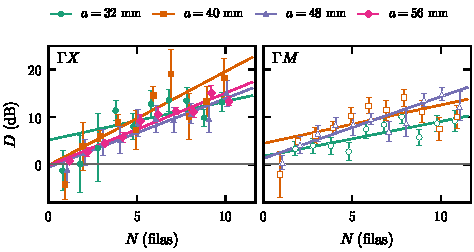
\includegraphics[width=\columnwidth]{figuras/fig3_profundidade.pdf}
  \caption{Profundidade $D$ em $f_B\pm10\,\%$ contra o número de filas, com a reta $D=\alpha N+b$
  ajustada para cada $a$ (declives na Tabela~\ref{tab:res}).}
  \label{fig:D}
\end{figure}
\begin{table}[t]
  \centering
  \caption{Resultados por bloco (média dos $N\ge4$) contra a PWE. Frequências em Hz;
  $\alpha$ em dB/fila. ${}^\dagger$\,O hiato não fecha. ${}^\ddagger$\,Só 14--38\,\% da janela
  $f_B\pm10\,\%$ está no hiato teórico: compara só ordens de grandeza.}
  \label{tab:res}
  \scriptsize\setlength{\tabcolsep}{1.7pt}
  \begin{tabular}{@{}llrrrrrrrrr@{}}
    \toprule
    & $a$ & $f_B$ & \multicolumn{3}{c}{$\finf$} & \multicolumn{3}{c}{$\fsup$} & \multicolumn{2}{c}{$\alpha$} \\
    \cmidrule(lr){4-6}\cmidrule(lr){7-9}\cmidrule(l){10-11}
    & mm & & medido & PWE & $z$ & medido & PWE & $z$ & medido & PWE \\
    \midrule
    $\GX$ & 32 & 5367 & $3806(84)$  & 3892 & 1,0 & $5923(191)$ & 6037 & 0,6 & $0{,}81(39)$ & 5,4 \\
          & 40 & 4294 & $3586(151)$ & 3387 & 1,3 & $5117(227)$ & 4752 & 1,6 & $1{,}98(41)$ & 4,0 \\
          & 48 & 3578 & $2969(102)$ & 2988 & 0,2 & $4230(135)$ & 3880 & 2,6 & $1{,}45(29)$ & 2,8 \\
          & 56 & 3067 & $2917(62)$  & 2666 & 3,9 & $3722(124)$ & 3271 & 3,6 & $1{,}53(11)$ & 1,9 \\
    \midrule
    $\GM$ & 32 & 7584 & $5500(271)$ & 6180 & 2,5 & ---$^\dagger$ & 6990 & --- & $0{,}73(20)$ & $0{,}1^\ddagger$ \\
          & 40 & 6067 & $4557(173)$ & 5109 & 3,1 & $7149(410)$ & 5818 & 3,2 & $0{,}81(28)$ & $0{,}5^\ddagger$ \\
          & 48 & 5056 & $4040(93)$  & 4385 & 3,6 & ---$^\dagger$ & 4942 & --- & $1{,}30(17)$ & $0{,}6^\ddagger$ \\
    \bottomrule
  \end{tabular}
\end{table}

\emph{Bordos do hiato.} Em $\GX$ há um hiato bem definido para $N\ge4$ em todos os $a$
(Fig.~\ref{fig:T}); fecha em 27 das 28 medições com $N\ge4$. Os bordos estão na
Tabela~\ref{tab:res}: para $a\le48$\,mm $\finf$ concorda com a PWE dentro de $1{,}3\sigma$, e $\fsup$
dentro de $2{,}6\sigma$; para $a=56$\,mm ambos ficam acima ($z=3{,}9$ e $3{,}6$).

\emph{Dependência em $a$.} A reta $\fc=m/(2a)$ pela origem dá $m=339\pm15$\,m/s, compatível com
$c=343{,}5\pm0{,}6$\,m/s ($z=0{,}3$), mas com $\chi^2/\nu=15{,}4$ ($p=5\times10^{-10}$): em média o
centro está em $f_B$, mas não é proporcional a $1/a$. A reta livre descreve os pontos
($\chi^2/\nu=1{,}4$) com $m=229\pm20$\,m/s e ordenada $1283\pm231$\,Hz. Para $\finf$ o mesmo:
pela origem $m=278\pm20$\,m/s com $\chi^2/\nu=30$ (Apêndice~A). A PWE dá $\fc/f_B=0{,}925$--$0{,}968$.

\emph{Atenuação.} Em $\GX$ a profundidade cresce linearmente com $N$ (Fig.~\ref{fig:D}): para
$a=40$, 48 e 56\,mm a ordenada é $b=-0{,}2\pm2{,}0$, $-0{,}6\pm1{,}9$ e $-0{,}3\pm0{,}6$\,dB
(compatível com 0, como a Eq.~\eqref{eq:DN} prevê) e $\chi^2/\nu=0{,}3$--$1{,}4$. Para $a=32$\,mm, $D$
satura em ${\approx}13$\,dB a partir de $N=4$ e a reta dá $b=5{,}1\pm2{,}9$\,dB. O $\alpha$ medido é
15, 50, 53 e 80\,\% do da PWE para $a=32$--$56$\,mm.

\emph{Direção $\GM$.} $\finf$ está 8--11\,\% abaixo da PWE ($z=2{,}5$--$3{,}6$) e o hiato só fecha em
3/8, 5/8 e 4/8 das medições ($a=32$, 40, 48\,mm). A razão $\finf(\GM)/\finf(\GX)$ vale
$1{,}445(78)$, $1{,}271(72)$ e $1{,}360(56)$, contra $\sqrt2$ (Bragg; $z=0{,}4$, 2,0, 1,0) e
$1{,}59$, $1{,}51$, $1{,}47$ (PWE; $z=1{,}8$, 3,3, 1,9).
A sobreposição $\fsup(\GX)-\finf(\GM)$ medida é $423\pm331$, $560\pm286$ e $191\pm163$\,Hz,
menos de $2\sigma$ acima de zero; a PWE dá $-143$, $-357$ e $-505$\,Hz (sem hiato completo).

% =====================================================================================
\section{Discussão}
\emph{$\GX$.} A PWE de um cristal 2D infinito de hastes rígidas descreve o bordo de baixo para
$a\le48$\,mm sem parâmetros livres, e o hiato abaixo de $f_B$ para $a=32$\,mm ($f\!f=0{,}24$) confirma
o abrandamento do som pelos tijolos. É isso que faz a reta pela origem falhar: o declive
$339\pm15$\,m/s seria ``a velocidade do som'' se o hiato estivesse sempre em $f_B$, mas o $\chi^2/\nu$
mostra que não está. A tendência medida em $\fc/f_B$ é mais forte do que a da PWE, sobretudo por
$a=56$\,mm, onde o hiato teórico tem só 600\,Hz, comparável à suavização de $1/6$ de oitava
(${\approx}350$\,Hz a 3\,kHz), e os cruzamentos de um limiar fixo deixam de coincidir com os bordos
das bandas. O bloco $a=40$\,mm misturou duas sessões, daí a maior incerteza sistemática.

\emph{Atenuação.} $D\propto N$ com $b\approx0$ é a assinatura da onda de Bloch evanescente~\cite{sanchez1998}. Mas o
cristal tem 3,8\,cm de altura e 4 colunas de largura: há som que passa por cima e pelos lados, o
que impõe um teto de ${\approx}13$--$15$\,dB. Quanto maior o $\alpha$ teórico, mais cedo se chega ao
teto: por isso a fração medida/teoria cresce de 15\,\% ($a=32$) para 80\,\% ($a=56$).

\emph{$\GM$.} Com a fonte a ${\sim}70$\,cm e o cristal estreito, chega ao microfone som que atravessa o
cristal obliquamente, perto de $\GX$, cujo hiato está mais abaixo: $T$ começa a descer antes do
hiato de $\GM$ e $\finf$ sai baixo. Acima de $f_B$ as filas, de período $L=\sqrt2a$, difratam para
os lados a partir de $c/L=f_B$ e o som deixa de chegar ao microfone no eixo; o hiato fica ``aberto''.
Pelas mesmas razões a sobreposição medida não prova um hiato completo.

\emph{Limitações.} A referência domina o erro: mexer 1\,cm na coluna ou no microfone muda o espectro
vários dB, e a ondulação de $T$ (0,5--8\,dB) é muito maior do que a dispersão das repetições. Uma tampa
rígida, um cristal mais largo e remontagens repetidas reduziriam e mediriam estes efeitos.

% =====================================================================================
\section{Conclusão}
Um cristal de LEGO com $a=32$--$56$\,mm tem um hiato de Bragg em $\GX$ cujo bordo de baixo concorda
com a PWE dentro de $1{,}3\sigma$ para $a\le48$\,mm, e que não escala como $1/a$ por causa da fração
de enchimento. A atenuação é linear em $N$, $\alpha\approx1{,}5$--$2$\,dB/fila, limitada a
${\approx}15$\,dB pelo som que contorna o cristal. Em $\GM$ o hiato aparece cerca de $\sqrt2$ acima,
mas o bordo de baixo fica 8--11\,\% abaixo da PWE e o hiato não fecha, por propagação oblíqua e
difração lateral; não há evidência de hiato completo.

\begingroup
\scriptsize
\begin{thebibliography}{9}\setlength{\itemsep}{0pt}\setlength{\parsep}{0pt}
\bibitem{martinez1995} R.~Martínez-Sala \emph{et al.}, Nature \textbf{378}, 241 (1995).
\bibitem{kushwaha1993} M.~S.~Kushwaha \emph{et al.}, Phys.\ Rev.\ Lett.\ \textbf{71}, 2022 (1993).
\bibitem{sanchez1998} J.~V.~Sánchez-Pérez \emph{et al.}, Phys.\ Rev.\ Lett.\ \textbf{80}, 5325 (1998).
\bibitem{krokhin2003} A.~A.~Krokhin, J.~Arriaga, L.~N.~Gumen, Phys.\ Rev.\ Lett.\ \textbf{91}, 264302 (2003).
\bibitem{welch1967} P.~D.~Welch, IEEE Trans.\ Audio Electroacoust.\ \textbf{15}, 70 (1967).
\bibitem{bevington} P.~R.~Bevington, D.~K.~Robinson, \emph{Data Reduction and Error Analysis for the
  Physical Sciences}, McGraw-Hill (2003).
\end{thebibliography}
\endgroup

% =====================================================================================
%  APÊNDICE (não conta para as 2 páginas)
% =====================================================================================
\clearpage
\onecolumn
\appendix
\renewcommand{\thesection}{\Alph{section}}
\renewcommand{\thefigure}{\Alph{section}\arabic{figure}}
\setcounter{figure}{0}
\renewcommand{\thetable}{A\arabic{table}}
\setcounter{table}{0}
\small

\section{Dados e medições adicionais}
\begin{figure}[h]
  \centering
  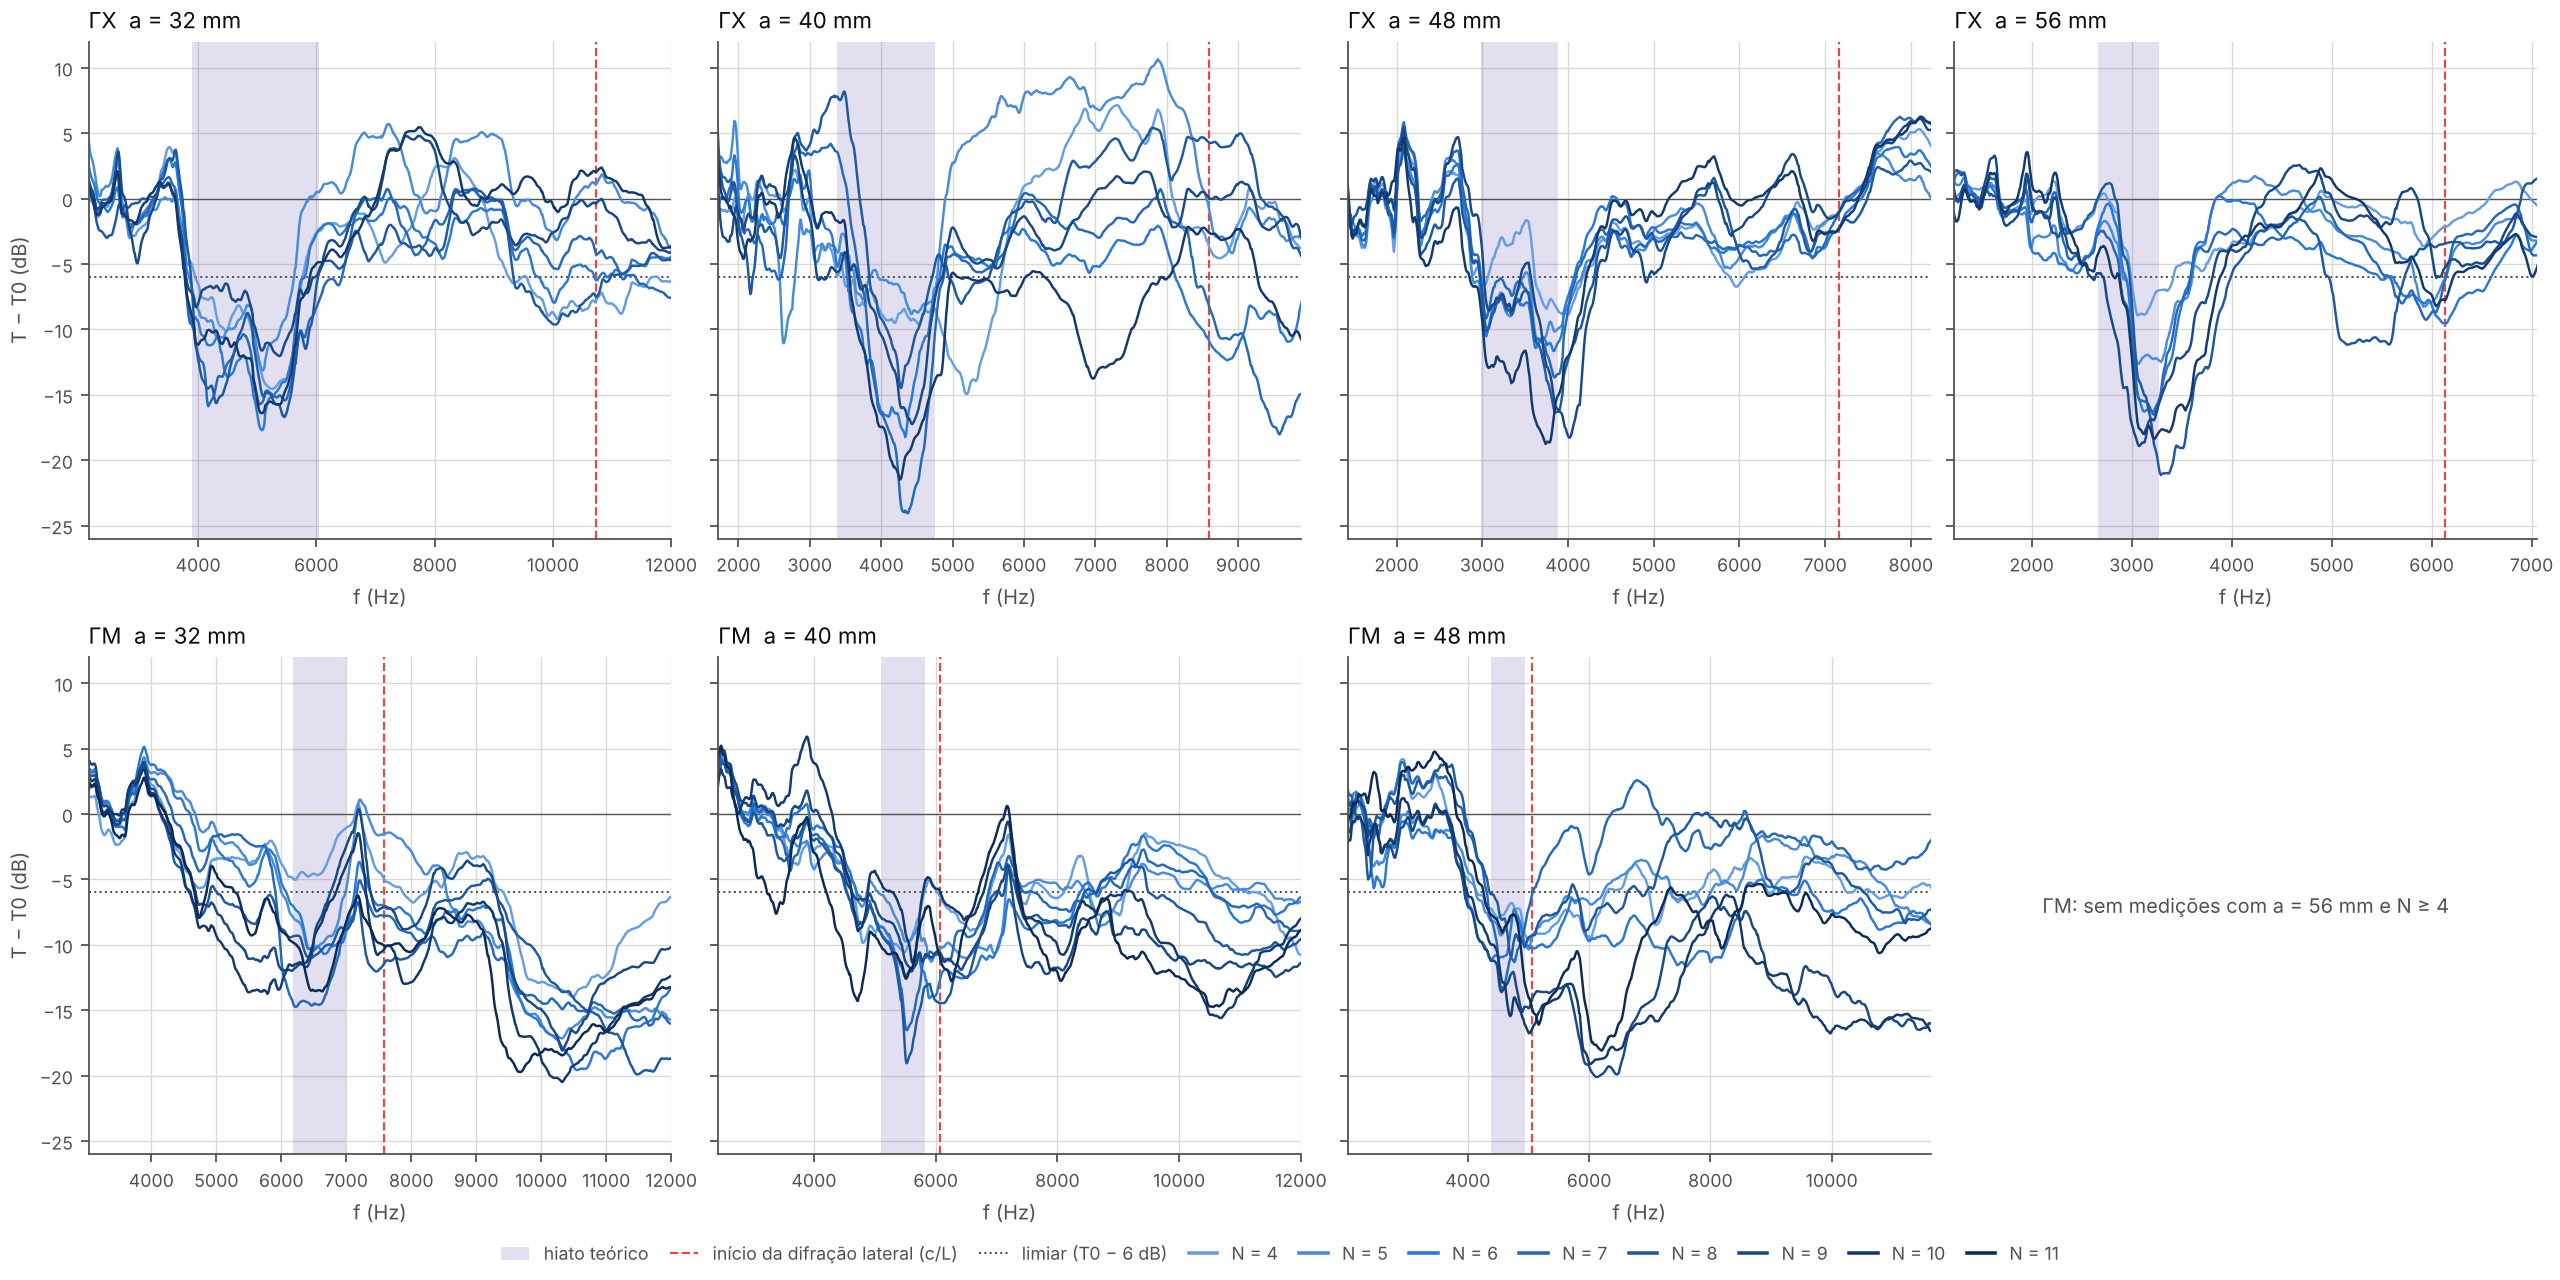
\includegraphics[width=\textwidth]{figuras/teoria_vs_medido.png}
  \caption{$T-T_0$ para todos os blocos com $N\ge4$ (cima: $\GX$; baixo: $\GM$). Faixa: hiato da PWE;
  vermelho tracejado: início da difração lateral, $c/L$; ponteado: limiar $T_0-6$\,dB.
  Em $\GM$ não há medições com $a=56$\,mm e $N\ge4$.}
\end{figure}
\begin{figure}[h]
  \centering
  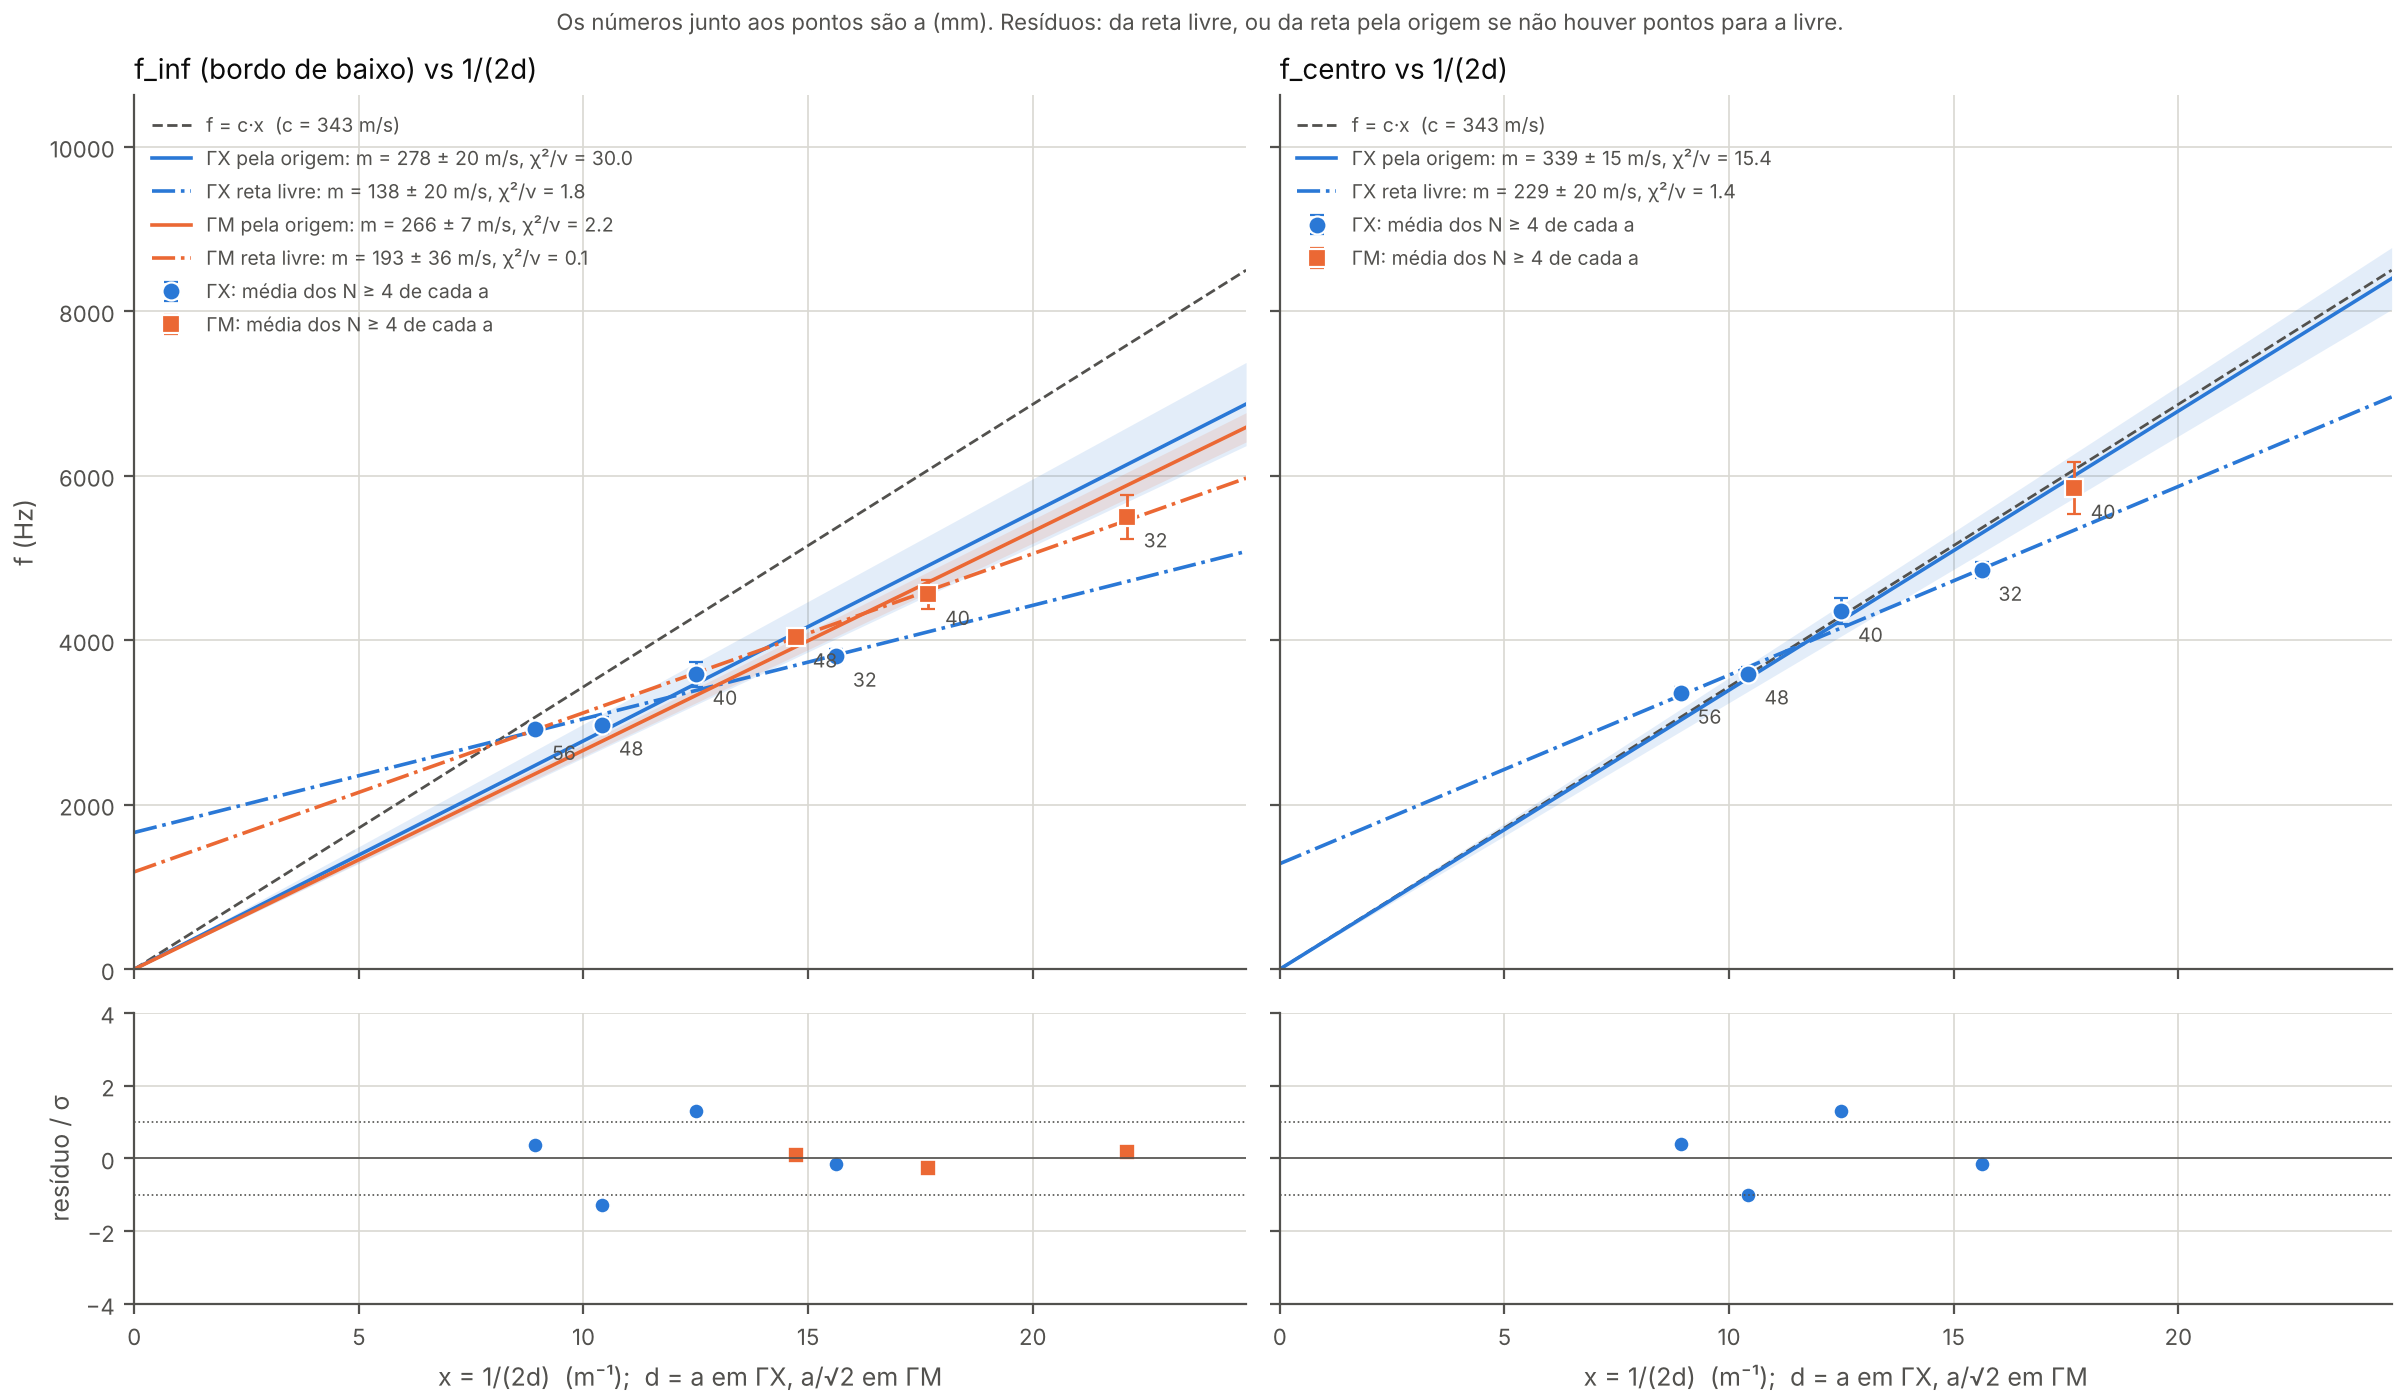
\includegraphics[width=0.92\textwidth]{figuras/f_vs_1_2d.png}
  \caption{$\finf$ e $\fc$ (média dos $N\ge4$ de cada $a$) contra $x=1/(2d)$, com a reta pela origem
  e a reta livre; em baixo, resíduos normalizados. Tracejado: $f=c\,x$.}
\end{figure}
\begin{figure}[h]
  \centering
  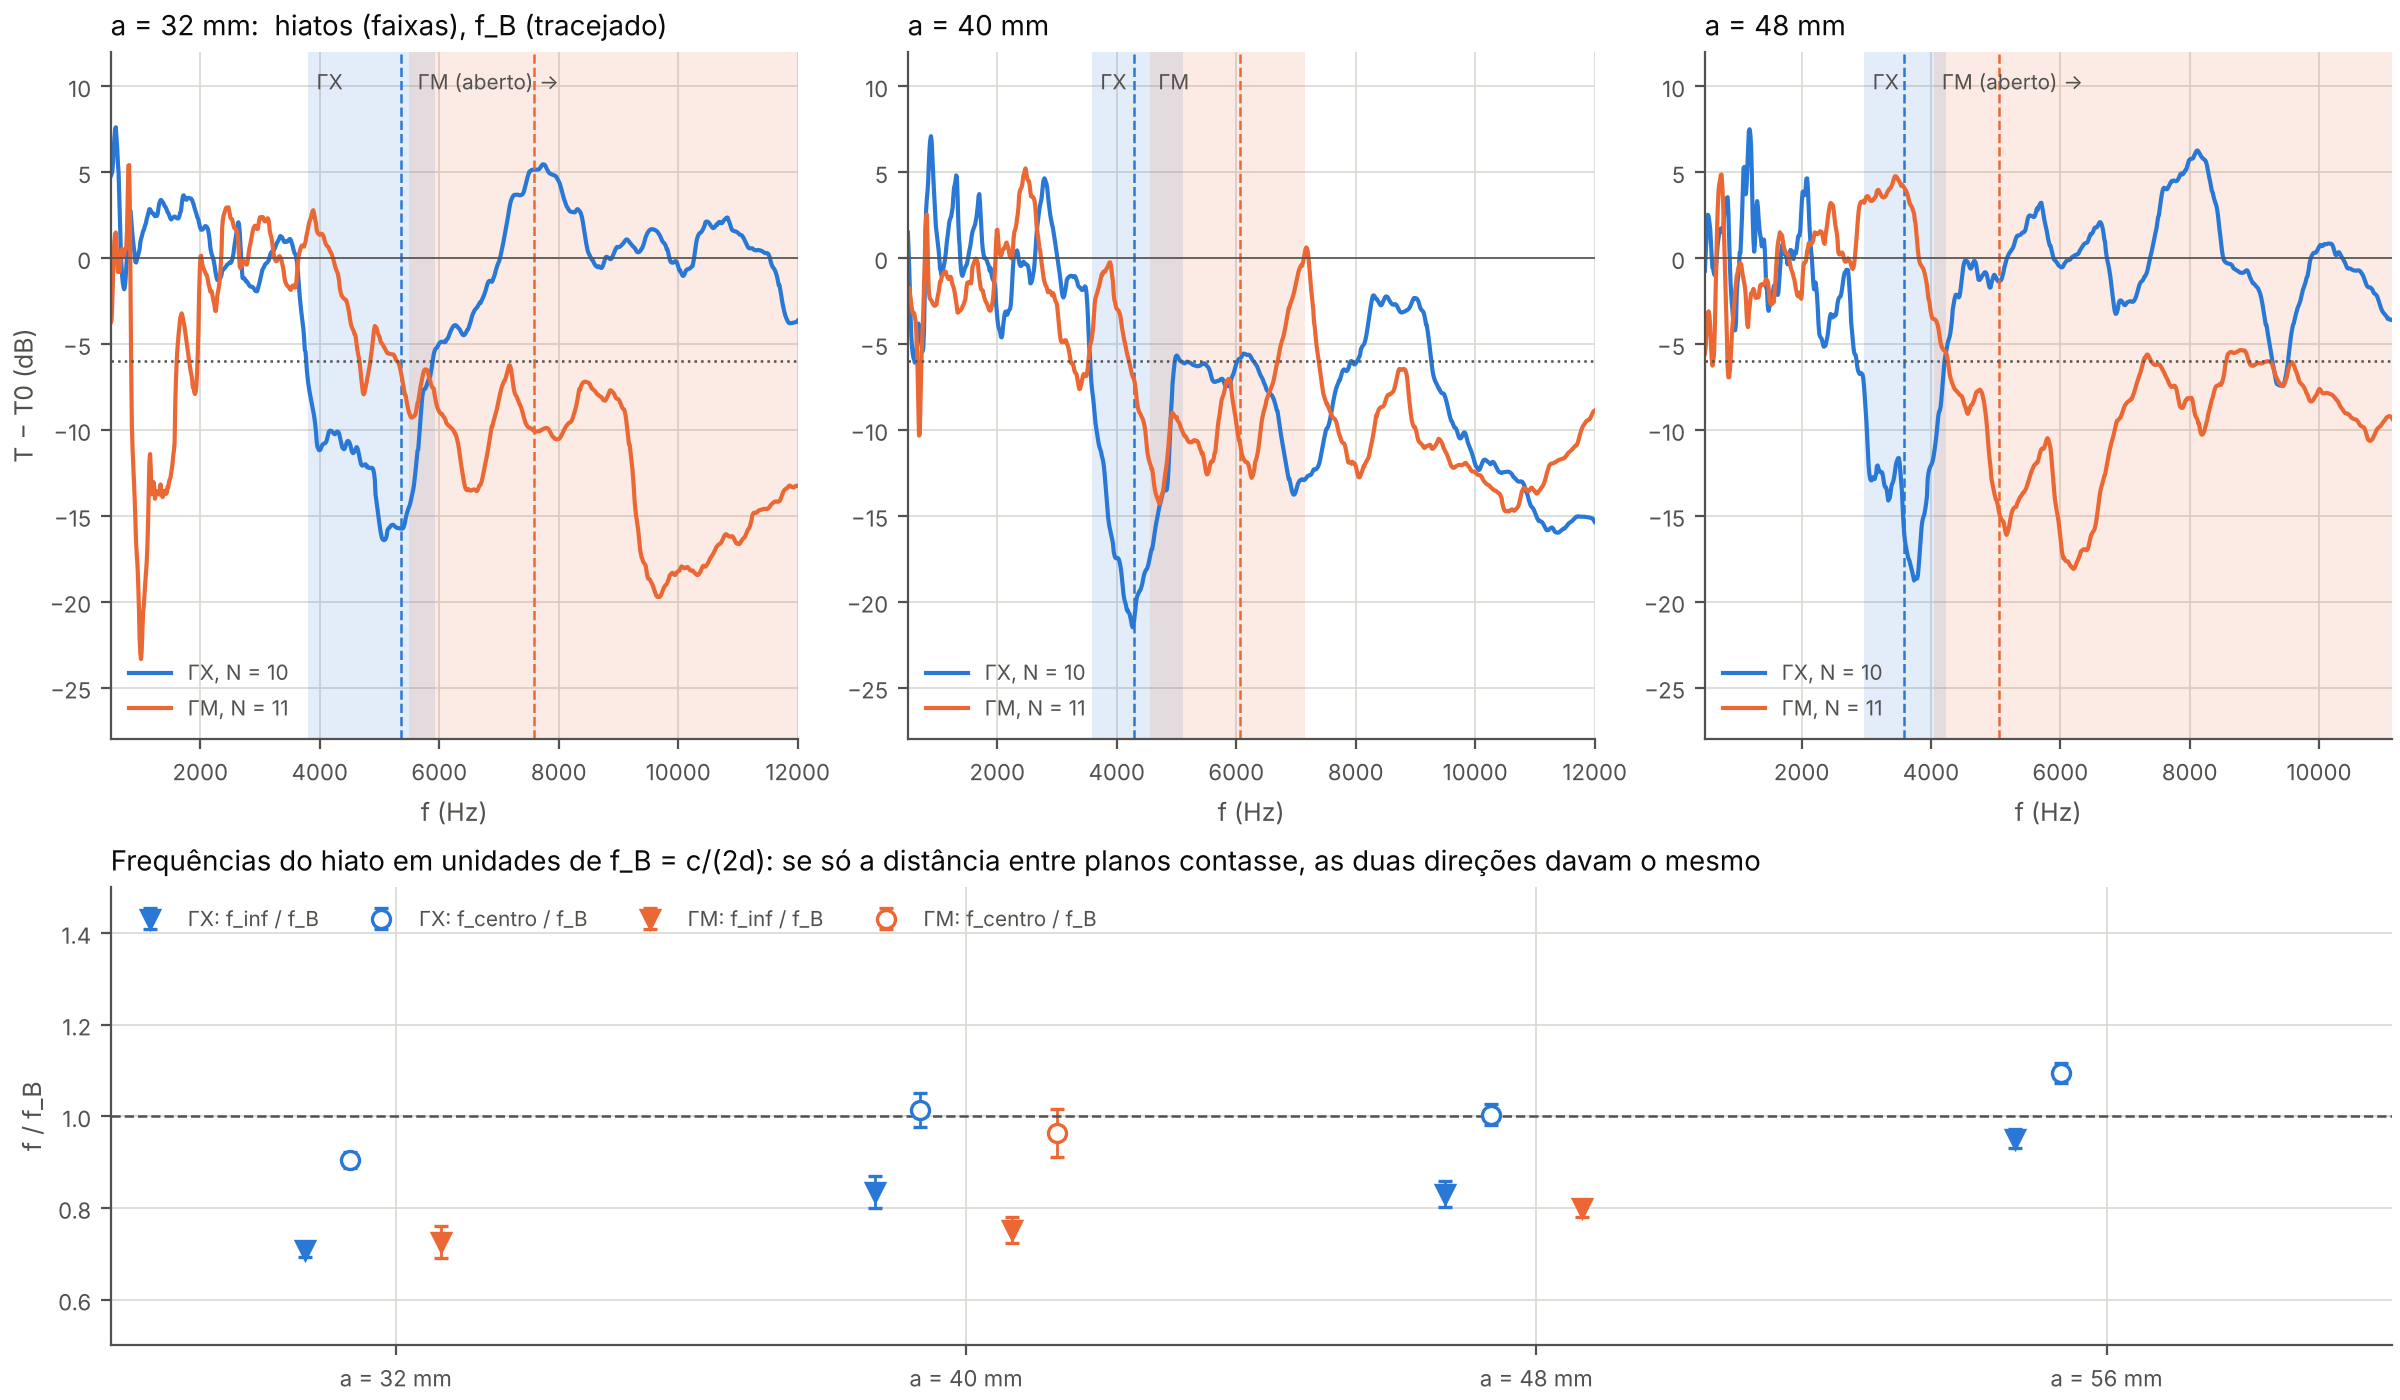
\includegraphics[width=0.92\textwidth]{figuras/comparacao_GX_GM.png}
  \caption{Cima: $\GX$ ($N=10$) e $\GM$ ($N=11$) para o mesmo $a$, com os hiatos medidos (faixas) e
  $f_B$ (tracejado). Baixo: $\finf/f_B$ e $\fc/f_B$ nas duas direções.}
\end{figure}

\clearpage
{\footnotesize
\setlength{\tabcolsep}{4pt}
\begin{longtable}{@{}llrllrrrrl@{}}
  \caption{Todas as medições. ``ond.'': ondulação de $T$ na banda de controlo (dB);
  ``inv.'': não entra nos ajustes; ``$k/5$ rep.'': repetições aproveitadas; ``ref.\ outro $a$'':
  referência da mesma sessão mas de outro bloco. Incerteza total
  $\sigma^2=\sigma_\text{est}^2+\sigma_\text{ond}^2+\sigma_\text{ref}^2(+\sigma_\text{res}^2)$.
  Em \texttt{tabela.csv} estão também as componentes.}\\
  \toprule
  dir & $a$ (mm) & $N$ & dia & referência & ond. & $D$ (dB) & $\finf$ (Hz) & $\fsup$ (Hz) & notas \\
  \midrule\endfirsthead
  \toprule
  dir & $a$ (mm) & $N$ & dia & referência & ond. & $D$ (dB) & $\finf$ (Hz) & $\fsup$ (Hz) & notas \\
  \midrule\endhead
  \bottomrule\endfoot
  $\Gamma X$ & 32 & 1 & 10-01 & ref\_a32 & 4.2 & $-1.3\pm4.3$ & --- & --- &  \\
$\Gamma X$ & 32 & 2 & 10-01 & ref\_a32 & 6.2 & $0.1\pm6.0$ & --- & --- &  \\
$\Gamma X$ & 32 & 3 & 10-01 & ref\_a32 & 7.6 & $3.5\pm7.2$ & $5529\pm889$ & $5609\pm599$ &  \\
$\Gamma X$ & 32 & 4 & 10-01 & ref\_a32 & 1.7 & $11.4\pm2.1$ & $3947\pm195$ & $5768\pm1747$ & 4/5 rep. \\
$\Gamma X$ & 32 & 5 & 10-01 & ref\_a32 & 1.8 & $8.0\pm2.7$ & $3846\pm133$ & $5622\pm161$ &  \\
$\Gamma X$ & 32 & 6 & 10-01 & ref\_a32 & 2.2 & $12.7\pm2.8$ & $3795\pm67$ & $5802\pm109$ &  \\
$\Gamma X$ & 32 & 7 & 10-01 & ref\_a32 & 1.7 & $13.5\pm2.3$ & $3781\pm70$ & $6431\pm165$ &  \\
$\Gamma X$ & 32 & 8 & 10-01 & ref\_a32 & 2.1 & $13.4\pm2.8$ & $3880\pm91$ & $6028\pm181$ &  \\
$\Gamma X$ & 32 & 9 & 10-01 & ref\_a32 & 1.5 & $9.9\pm1.8$ & $3794\pm79$ & $5981\pm893$ &  \\
$\Gamma X$ & 32 & 10 & 10-01 & ref\_a32 & 1.6 & $13.1\pm2.0$ & $3773\pm78$ & $5890\pm919$ & 4/5 rep. \\
$\Gamma X$ & 40 & 1 & 10-06 & ref\_a56 & 3.1 & $-4.2\pm3.1$ & --- & --- & 4/5 rep., ref. outro $a$ \\
$\Gamma X$ & 40 & 2 & 10-06 & ref\_a56 & 5.4 & $3.9\pm5.1$ & $4538\pm944$ & $4713\pm254$ & ref. outro $a$ \\
$\Gamma X$ & 40 & 3 & 10-06 & ref\_a56 & 1.0 & $6.0\pm1.2$ & $3196\pm330$ & $4832\pm126$ & 4/5 rep., ref. outro $a$ \\
$\Gamma X$ & 40 & 4 & 10-06 & ref\_a56 & 1.2 & $8.9\pm1.6$ & $3474\pm168$ & $5677\pm114$ & ref. outro $a$ \\
$\Gamma X$ & 40 & 5 & 10-06 & ref\_a56 & 4.2 & $7.2\pm4.1$ & $3625\pm327$ & $4783\pm163$ & ref. outro $a$ \\
$\Gamma X$ & 40 & 6 & 10-06 & ref\_a56 & 2.0 & $14.5\pm2.0$ & $3525\pm122$ & $4818\pm271$ & ref. outro $a$ \\
$\Gamma X$ & 40 & 7 & 10-01 & ref\_a40 & 4.4 & $19.0\pm5.3$ & $3696\pm157$ & $4875\pm185$ &  \\
$\Gamma X$ & 40 & 8 & 10-01 & ref\_a40 & 4.7 & $10.1\pm4.8$ & $3833\pm213$ & $5510\pm462$ &  \\
$\Gamma X$ & 40 & 9 & 10-01 & ref\_a40 & 1.9 & $13.2\pm3.2$ & $3669\pm330$ & $4854\pm111$ &  \\
$\Gamma X$ & 40 & 10 & 10-01 & ref\_a40 & 2.2 & $18.2\pm4.1$ & $3556\pm101$ & --- & não fecha \\
$\Gamma X$ & 48 & 1 & 10-06 & ref\_a48 & 1.9 & $-1.1\pm2.7$ & --- & --- &  \\
$\Gamma X$ & 48 & 2 & 10-06 & ref\_a48 & 2.4 & $2.5\pm2.7$ & --- & --- & 4/5 rep. \\
$\Gamma X$ & 48 & 3 & 10-06 & ref\_a48 & 2.3 & $4.6\pm2.7$ & $3600\pm502$ & $3770\pm1598$ &  \\
$\Gamma X$ & 48 & 4 & 10-06 & ref\_a48 & 2.3 & $5.2\pm2.9$ & $3613\pm568$ & $4173\pm364$ &  \\
$\Gamma X$ & 48 & 5 & 10-06 & ref\_a48 & 2.7 & $8.7\pm2.8$ & $2883\pm125$ & $4157\pm260$ &  \\
$\Gamma X$ & 48 & 6 & 10-06 & ref\_a48 & 2.5 & $9.6\pm2.9$ & $2970\pm100$ & $4071\pm161$ & 4/5 rep. \\
$\Gamma X$ & 48 & 7 & 10-06 & ref\_a48 & 2.0 & $9.4\pm2.6$ & $2982\pm98$ & $4093\pm130$ & 4/5 rep. \\
$\Gamma X$ & 48 & 8 & 10-06 & ref\_a48 & 2.0 & $10.7\pm2.1$ & $2974\pm83$ & $4306\pm112$ &  \\
$\Gamma X$ & 48 & 9 & 10-06 & ref\_a48 & 2.3 & $9.6\pm2.8$ & $3019\pm79$ & $4332\pm96$ &  \\
$\Gamma X$ & 48 & 10 & 10-06 & ref\_a48 & 2.8 & $15.0\pm2.7$ & $2850\pm135$ & $4210\pm123$ &  \\
$\Gamma X$ & 56 & 1 & 10-06 & ref\_a56 & 0.8 & $0.7\pm0.7$ & --- & --- &  \\
$\Gamma X$ & 56 & 2 & 10-06 & ref\_a56 & 1.1 & $2.7\pm1.0$ & --- & --- & 4/5 rep. \\
$\Gamma X$ & 56 & 3 & 10-06 & ref\_a56 & 0.5 & $4.4\pm0.5$ & $3018\pm50$ & $3142\pm230$ &  \\
$\Gamma X$ & 56 & 4 & 10-06 & ref\_a56 & 1.1 & $5.7\pm1.0$ & $2993\pm75$ & $3418\pm200$ &  \\
$\Gamma X$ & 56 & 5 & 10-06 & ref\_a56 & 1.6 & $9.1\pm1.5$ & $2912\pm72$ & $3607\pm133$ & 4/5 rep. \\
$\Gamma X$ & 56 & 6 & 10-06 & ref\_a56 & 1.6 & $10.6\pm1.5$ & $2941\pm56$ & $3587\pm98$ & 4/5 rep. \\
$\Gamma X$ & 56 & 7 & 10-06 & ref\_a56 & 0.8 & $11.3\pm0.7$ & $2884\pm46$ & $3593\pm77$ &  \\
$\Gamma X$ & 56 & 8 & 10-06 & ref\_a56 & 1.3 & $11.0\pm1.2$ & $2979\pm47$ & $3993\pm103$ &  \\
$\Gamma X$ & 56 & 9 & 10-06 & ref\_a56 & 1.5 & $15.1\pm1.5$ & $2595\pm266$ & $3809\pm215$ &  \\
$\Gamma X$ & 56 & 10 & 10-06 & ref\_a56 & 1.0 & $13.3\pm0.9$ & $2821\pm58$ & $3886\pm85$ &  \\
$\Gamma M$ & 32 & 2 & 10-13 & ref\_a32 & 1.6 & $3.3\pm1.5$ & $6288\pm297$ & $6883\pm150$ &  \\
$\Gamma M$ & 32 & 3 & 10-13 & ref\_a32 & 1.7 & $4.0\pm1.6$ & $5950\pm96$ & $6953\pm128$ &  \\
$\Gamma M$ & 32 & 4 & 10-13 & ref\_a32 & 2.0 & $3.9\pm1.8$ & $7871\pm1018$ & $8223\pm817$ & 4/5 rep. \\
$\Gamma M$ & 32 & 5 & 10-13 & ref\_a32 & 2.0 & $2.7\pm1.9$ & $6005\pm2114$ & $6989\pm120$ &  \\
$\Gamma M$ & 32 & 6 & 10-13 & ref\_a32 & 2.0 & $7.4\pm1.9$ & $6076\pm179$ & --- & não fecha \\
$\Gamma M$ & 32 & 7 & 10-13 & ref\_a32 & 1.8 & $8.4\pm1.6$ & $5910\pm73$ & --- & 4/5 rep., não fecha \\
$\Gamma M$ & 32 & 8 & 10-13 & ref\_a32 & 1.6 & $10.0\pm1.5$ & $4603\pm189$ & --- & não fecha \\
$\Gamma M$ & 32 & 9 & 10-13 & ref\_a32 & 1.9 & $5.7\pm1.8$ & $4680\pm206$ & $8281\pm309$ &  \\
$\Gamma M$ & 32 & 10 & 10-13 & ref\_a32 & 1.9 & $8.7\pm1.8$ & $4581\pm141$ & --- & não fecha \\
$\Gamma M$ & 32 & 11 & 10-13 & ref\_a32 & 2.4 & $9.2\pm2.2$ & $4664\pm353$ & --- & não fecha \\
$\Gamma M$ & 40 & 1 & 10-13 & ref\_a40\_fim & 5.3 & $-2.1\pm4.9$ & --- & --- &  \\
$\Gamma M$ & 40 & 2 & 10-13 & ref\_a40\_fim & 1.4 & $4.8\pm1.3$ & $6260\pm302$ & $6794\pm1291$ &  \\
$\Gamma M$ & 40 & 3 & 10-13 & ref\_a40\_fim & 1.9 & $6.1\pm1.7$ & $4712\pm335$ & $5756\pm593$ & 4/5 rep. \\
$\Gamma M$ & 40 & 4 & 10-13 & ref\_a40\_fim & 1.4 & $7.7\pm1.3$ & $4633\pm101$ & --- & 4/5 rep., não fecha \\
$\Gamma M$ & 40 & 5 & 10-13 & ref\_a40\_fim & 1.9 & $10.2\pm1.7$ & $4695\pm445$ & $7151\pm209$ &  \\
$\Gamma M$ & 40 & 6 & 10-13 & ref\_a40\_fim & 1.9 & $12.4\pm1.7$ & $4706\pm213$ & $8699\pm493$ &  \\
$\Gamma M$ & 40 & 7 & 10-13 & ref\_a40\_fim & 2.3 & $11.4\pm2.2$ & $4535\pm210$ & $6865\pm1507$ &  \\
$\Gamma M$ & 40 & 8 & 10-13 & ref\_a40\_fim & 2.0 & $14.1\pm1.8$ & $4544\pm175$ & $8655\pm429$ &  \\
$\Gamma M$ & 40 & 9 & 10-13 & ref\_a40\_fim & 2.5 & $11.1\pm2.3$ & $4624\pm342$ & --- & não fecha \\
$\Gamma M$ & 40 & 10 & 10-13 & ref\_a40\_fim & 2.6 & $7.4\pm2.4$ & $4616\pm184$ & --- & não fecha \\
$\Gamma M$ & 40 & 11 & 10-13 & ref\_a40\_fim & 2.6 & $9.9\pm2.4$ & $4206\pm165$ & $6696\pm177$ & 4/5 rep. \\
$\Gamma M$ & 48 & 1 & 10-12 & ref\_a48\_fim & 1.4 & $0.4\pm1.5$ & --- & --- &  \\
$\Gamma M$ & 48 & 2 & 10-12 & ref\_a48\_fim & 1.3 & $4.2\pm1.8$ & $5838\pm656$ & --- & 4/5 rep. \\
$\Gamma M$ & 48 & 3 & 10-12 & ref\_a48\_fim & 1.2 & $6.5\pm1.7$ & $3896\pm112$ & --- &  \\
$\Gamma M$ & 48 & 4 & 10-12 & ref\_a48\_fim & 1.3 & $8.3\pm1.6$ & $4148\pm215$ & $6287\pm557$ &  \\
$\Gamma M$ & 48 & 5 & 10-12 & ref\_a48\_fim & 1.9 & $8.5\pm2.3$ & $4131\pm176$ & $6232\pm769$ &  \\
$\Gamma M$ & 48 & 6 & 10-12 & ref\_a48\_fim & 1.0 & $9.6\pm1.2$ & $3966\pm61$ & --- & não fecha \\
$\Gamma M$ & 48 & 7 & 10-12 & ref\_a48\_fim & 1.7 & $7.0\pm2.2$ & $4314\pm76$ & $5068\pm144$ &  \\
$\Gamma M$ & 48 & 8 & 10-12 & ref\_a48\_fim & 2.7 & $8.7\pm2.7$ & $4360\pm236$ & $6941\pm973$ &  \\
$\Gamma M$ & 48 & 9 & 10-12 & ref\_a48\_fim & 0.9 & $13.6\pm1.3$ & $3945\pm50$ & --- & não fecha \\
$\Gamma M$ & 48 & 10 & 10-12 & ref\_a48\_fim & 1.2 & $14.8\pm1.4$ & $3990\pm85$ & --- & não fecha \\
$\Gamma M$ & 48 & 11 & 10-12 & ref\_a48\_fim & 2.1 & $12.2\pm3.0$ & $4260\pm188$ & --- & não fecha \\
\end{longtable}}

\section{Calibrações e derivações}
\emph{Velocidade do som.} $c(T)=331{,}3\sqrt{1+T/273{,}15}$\,m/s, $\sigma_c=c\,\sigma_T/[2(273{,}15+T)]=0{,}6$\,m/s
para $\sigma_T=1\,^\circ$C.

\emph{Onda plana.} A frente esférica chega às pontas de um cristal de largura $w\approx4a$ atrasada de
$w^2/8\ell$ ($\ell$: distância coluna--cristal). Exigindo $\le\lambda/10$ no bordo de cima do hiato
($\lambda\approx2a/1{,}2$) obtém-se $\ell\ge1{,}25\,w^2/\lambda$, isto é $38$--$67$\,cm para $a=32$--$56$\,mm;
para a coluna estéreo ($D_s\approx\confirmar{15}$\,cm entre altifalantes), o campo distante pede
$\ell>2D_s^2/\lambda\approx85$\,cm para $a=32$\,mm. As pontas do cristal veem a onda inclinada de
$\theta\approx\arctan(w/2\ell)\lesssim9^\circ$, o que desloca o hiato local de ${\lesssim}1\,\%$.

\emph{Expansão em ondas planas.} Com $\sigma=1/\rho$, $\eta=1/(\rho c^2)$ e
$p(\mathbf r)=e^{i\mathbf k\cdot\mathbf r}\sum_{\mathbf G}p_{\mathbf G}e^{i\mathbf G\cdot\mathbf r}$,
$\mathbf G=\tfrac{2\pi}{a}(m,n)$, a equação de onda dá, para cada $\mathbf k$, o problema de valores próprios
\begin{equation*}
  \sum_{\mathbf G'}\sigma(\mathbf G-\mathbf G')\,(\mathbf k+\mathbf G)\cdot(\mathbf k+\mathbf G')\,p_{\mathbf G'}
  =\omega^2\sum_{\mathbf G'}\eta(\mathbf G-\mathbf G')\,p_{\mathbf G'},
\end{equation*}
com, para uma haste quadrada de lado $s$,
$\sigma(\mathbf G)=(\sigma_\text{t}-\sigma_\text{ar})\,f\!f\,\operatorname{sinc}(G_xs/2)\operatorname{sinc}(G_ys/2)$
($\mathbf G\neq0$). Usam-se $15^2=225$ ondas (729 ondas mudam os bordos 0,1--0,4\,\%). Só contam os modos
simétricos em relação ao plano que contém a direção do som (os antissimétricos não são excitados por
uma onda que chega de frente). O hiato é $\finf=\max_k f_1(k)$, $\fsup=\min_k f_{n\ge2}(k)$, com $k$ de
$\Gamma$ a X ($|\mathbf k|=\pi/a$) ou de $\Gamma$ a M ($|\mathbf k|=\sqrt2\pi/a$). A atenuação vem do
problema inverso (dado $\omega$, sai $k$ complexo), $(k^2M_2+kM_1+M_0)\mathbf p=0$, linearizado num problema
de dimensão dupla; $\kappa$ é o menor $|\operatorname{Im}k|$. Com só as duas ondas $e^{\pm i\pi x/d}$,
$\fsup-\finf\propto|\sigma(2\pi/d)|$: o hiato alarga com a quantidade de tijolo por plano.

\emph{Meio efetivo.} A baixa frequência, $\kappa_\text{ef}=(1-f\!f)\kappa$ e
$\rho_\text{ef}\simeq\rho(1+f\!f)/(1-f\!f)$ (hastes rígidas), logo $c_\text{ef}=c/\sqrt{1+f\!f}$ e
$f_\text{hiato}\approx f_B/\sqrt{1+f\!f}=0{,}90$, $0{,}93$, $0{,}95$, $0{,}96\,f_B$ para $a=32$--$56$\,mm.

\emph{Hiato completo.} Há hiato em todas as direções se $\fsup(\GX)>\finf(\GM)$. Ao longo de $\GM$ a diagonal
do tijolo (22,3\,mm) ocupa quase toda a distância entre planos ($a/\sqrt2=22{,}6$\,mm para $a=32$\,mm): o meio
parece quase uniforme e o hiato de $\GM$ é estreito, pelo que a razão $\finf(\GM)/\finf(\GX)$ prevista é
$1{,}59$, $1{,}51$, $1{,}47$ (e não $\sqrt2$) e não há sobreposição para tijolos $2{\times}2$
(${-}7$\,Hz mesmo para $a=24$\,mm).

\emph{Incertezas da profundidade.} $D=T_0-M$; com $n_\text{base}=\log_2(0{,}70/0{,}35)/(1/6)=6$ e
$n_\text{jan}=\log_2(1{,}1/0{,}9)/(1/6)=1{,}74$ pontos independentes, e a variância da mediana $\pi/2$ vezes a
da média, $\operatorname{Var}D=(\tfrac{\pi}{2}\tfrac16+\tfrac{1}{1{,}74})\sigma^2$, i.e.
$\sigma_\text{ond}(D)=0{,}92\times$ondulação. A dispersão das referências usa pesos
$w_k=1/\text{ond}_k^2$: $\sigma_\text{ref}^2=\sum_kw_k(x_k-x_0)^2/\sum_kw_k$.

\emph{Ajustes.} Para $y=mx+b$ com $w_i=1/\sigma_i^2$:
$m=(SS_{xy}-S_xS_y)/\Delta$, $b=(S_{xx}S_y-S_xS_{xy})/\Delta$, $\sigma_m^2=S/\Delta$, $\sigma_b^2=S_{xx}/\Delta$,
$\Delta=SS_{xx}-S_x^2$~\cite{bevington}; incerteza em $x$ por $\sigma_{i,\text{ef}}^2=\sigma_{y,i}^2+(m\sigma_{x,i})^2$,
minimizando $\chi^2(m,b)$ numericamente. Se $\chi^2/\nu>1$, $\sigma\to\sqrt{\chi^2/\nu}\,\sigma$; nunca se
encolhem incertezas. As regressões foram verificadas contra \texttt{numpy.polyfit},
\texttt{scipy.optimize.curve\_fit} e \texttt{scipy.odr}.

\section{Código}
Repositório: \url{https://github.com/FM767/LFE-acoustics}.
\begin{itemize}[nosep,leftmargin=1.2em]
  \item \texttt{cristal\_simples/} e \texttt{cristal\_lego\_g/cristal\_lego\_g/}: apps de medição ($\GX$ e $\GM$;
  Python, \texttt{sounddevice}) com o plano de medição, controlo de qualidade e as gravações
  (\texttt{projeto/dados/<passo>/*.wav} + \texttt{meta.json}; medições repetidas em \texttt{\_antigos/}, que não contam).
  \item \texttt{cristal\_lego\_g/analise 2.0/}: análise conjunta das duas direções.
  \texttt{analise.py} (espectros, $T(f)$, grandezas, incertezas, ajustes), \texttt{teoria.py} (PWE),
  \texttt{graficos.py}, \texttt{app.py} (interface); resultados em \texttt{resultados/}
  (\texttt{resultados.txt}, \texttt{tabela.csv}, \texttt{ajustes.csv}, \texttt{teoria.txt}).
  Todas as equações, por ordem, em \texttt{EQUACOES.md}.
  \item \texttt{relatorio/}: este relatório. \texttt{fazer\_figuras.py} gera as Figs.~2--3 e a
  Tabela~A1 a partir de \texttt{dados\_figuras/}; \texttt{dados\_figuras/curvas\_T.py} recalcula as curvas
  da Fig.~2 a partir dos \texttt{.wav} (mesmo método, só \texttt{numpy}).
\end{itemize}
Parâmetros: \texttt{FS = 48000}, \texttt{NPERSEG = 4096}, banda 0,5--12\,kHz, troço 0,8--10,3\,s,
suavização $1/6$ de oitava, limiar 6\,dB, $\sigma_a=0{,}1$\,mm, $\sigma_T=1\,^\circ$C.

\section{Uso de IA}
\confirmar{Usámos o Claude (Anthropic) como assistente: no planeamento da experiência e na escolha dos
parâmetros, na escrita do código de medição e de análise (que revimos e testámos: as regressões foram
comparadas com bibliotecas independentes e a cobertura das incertezas por simulação) e na redação
deste relatório a partir dos ficheiros de resultados. A montagem, as medições, as decisões sobre o
que medir e a verificação dos números contra \texttt{resultados.txt} e \texttt{teoria.txt} foram feitas
por nós. [Rever e ajustar a descrição.]}

\end{document}
